\section{Methodology}
\begin{figure}[t]
    \centering
    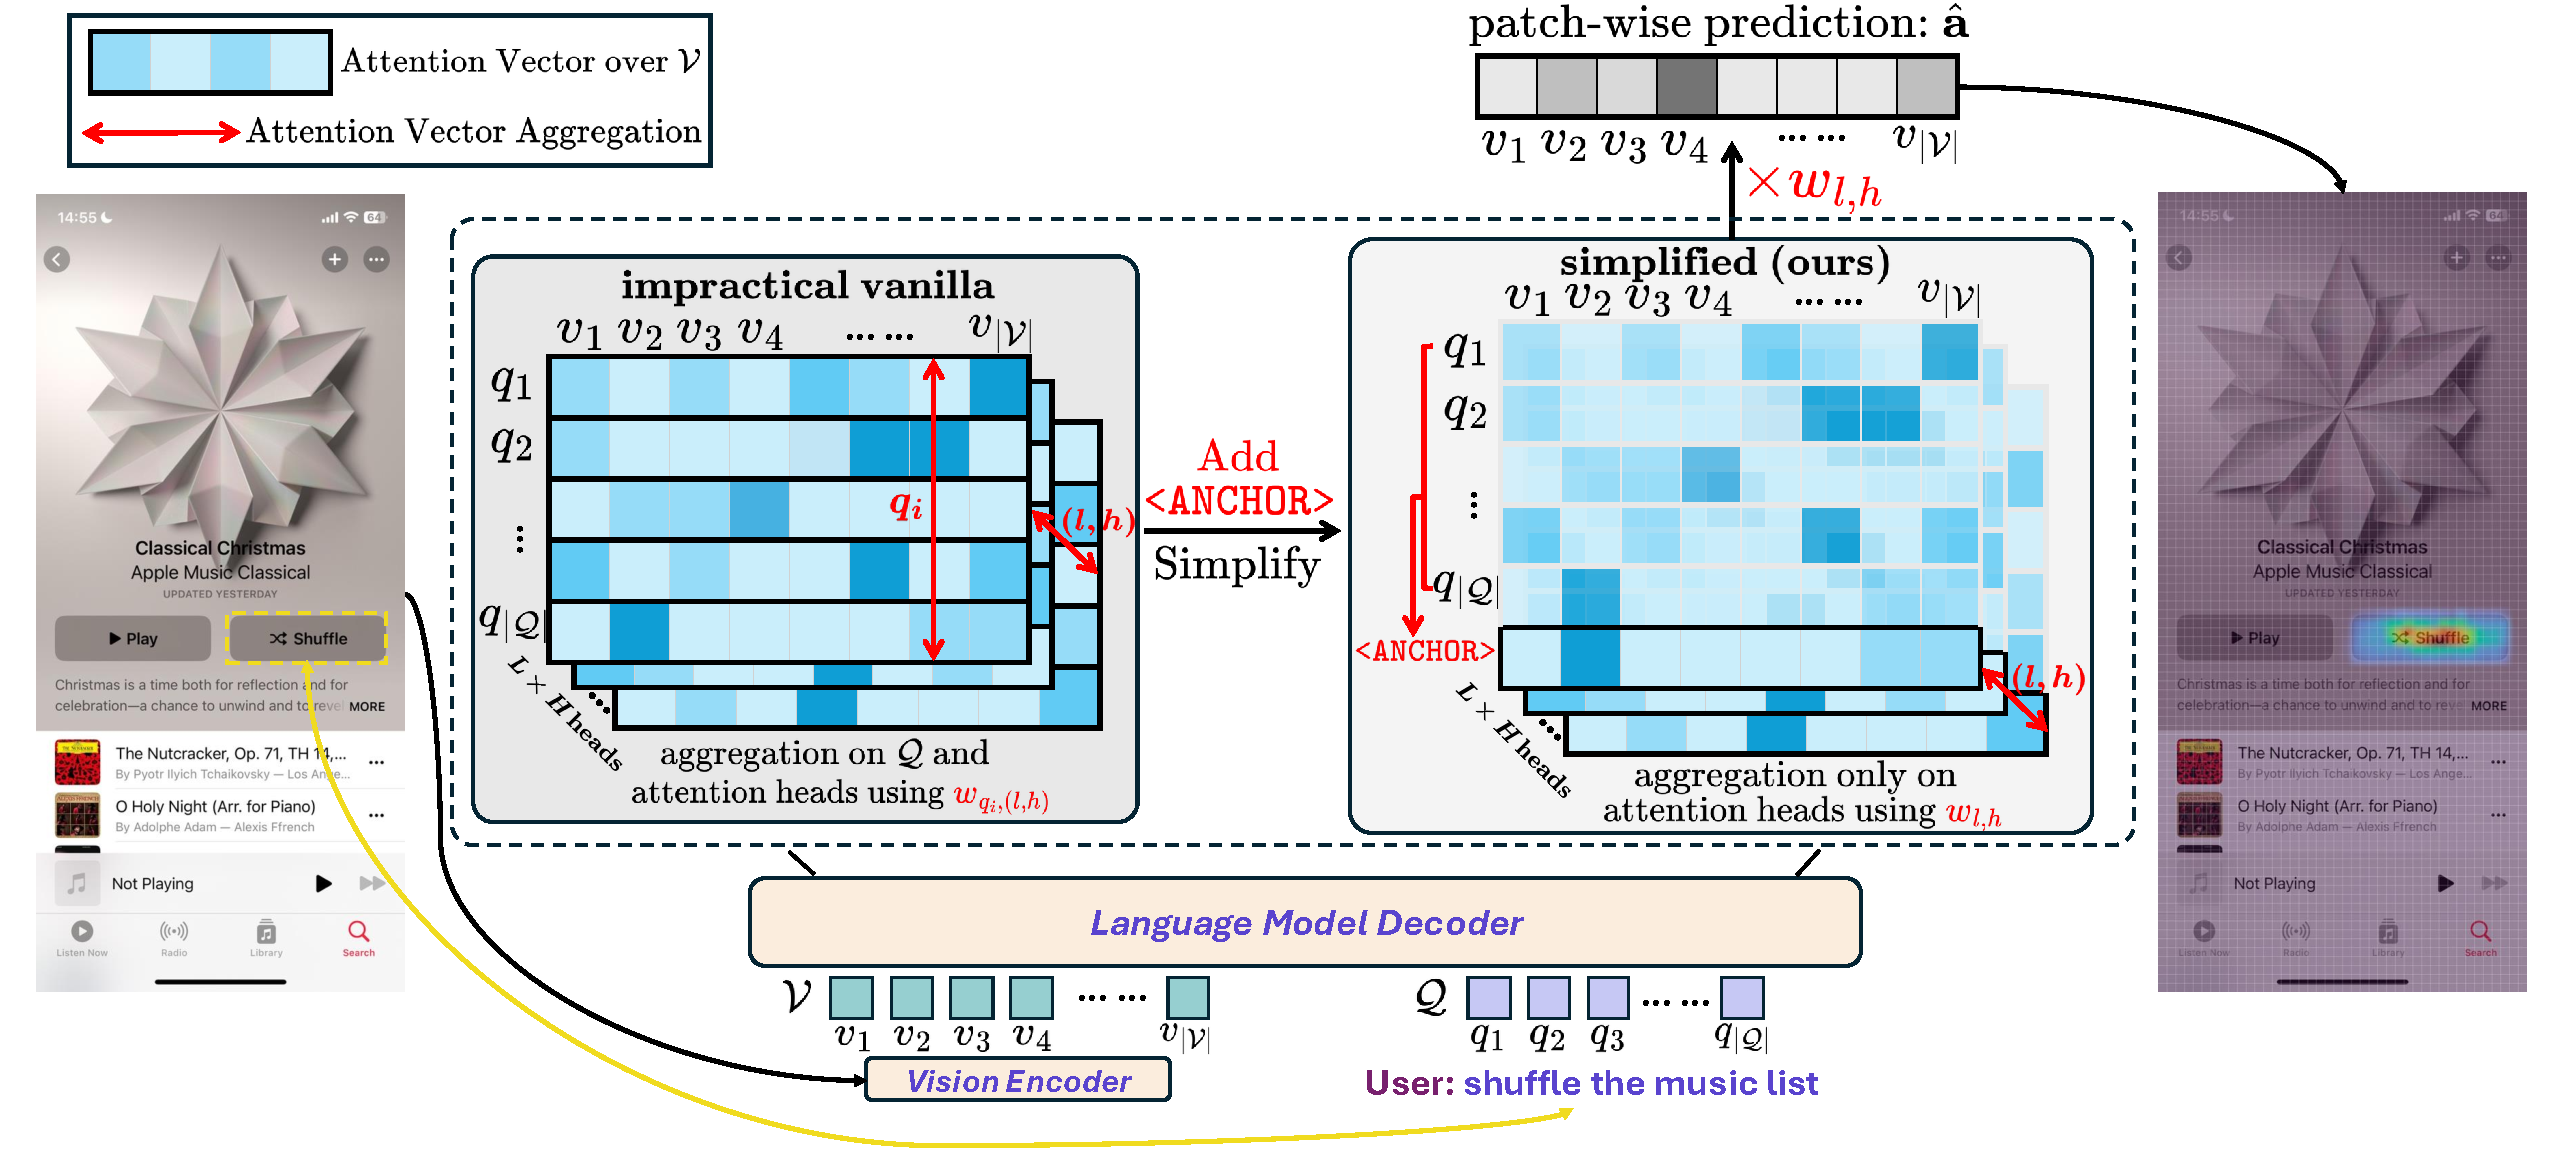
\includegraphics[width=0.95\linewidth]{fig/comparison.pdf}
    % \vspace{-1.2em}
    \caption{ With user query $\mathcal{Q}$, screenshot patches $\mathcal{V}$ and multi-head attentions $\{\mathbf{A}^{l,h}\}_{l\in[L],h\in[H]}$ from the MLLM, the vanilla attention grounding needs additional aggregation between all query tokens' grounding vectors. In our proposed simplified version, a special $\texttt{<ANCHOR>}$ token can learn to implicitly aggregate all query tokens. Then we aggregate grounding vectors of $\texttt{<ANCHOR>}$ token across layers and heads with carefully designed weights to produce the patch-wise predictions.} 
    % \vspace{-1.5em}
\label{fig:comparison_example}
\end{figure}
% \noindent
\method{} formulates GUI grounding as the attention supervision: it uses the MLLM’s intrinsic multi-head attention maps across layers as grounding indicators, instead of coordinate tokens, and directly supervises these attention maps without introducing additional grounding modules.
As illustrated in \cref{sec:pre}, within each attention head of the MLLM, the \textbf{patch-level attention vector} from a single text token (of the user query) to all visual tokens indicates the relevance of each visual patch to the target grounding region, naturally serving as grounding cues. 
\method{} fully exploits the attention vectors from the entire text sequence and all attention heads in a simple but precise way: adding a special representative token for query-level aggregation (\cref{sec:pre}) and adaptive head-wise reweighting based on multimodal importance (\cref{sec:head_agg}).
\subsection{Intrinsic Attention for GUI Grounding with an Anchor Token} \label{sec:pre}
\paragraph{Preliminaries on Multi-Head Self-Attention (MHSA).}
For each layer $1\leq l \leq L$ of MLLMs, each head $1\leq h \leq H$ computes the attention map $\mathbf{A}^{l,h}$ from preceding layer's embeddings $\mathbf{H}^{l-1}\in\mathbb{R}^{d}$ via $\mathbf{A}^{l,h}=\operatorname{softmax}\left(\mathbf{Q}^{l,h} \mathbf{K}^{l,h^{\top}} / \sqrt{d_h}+\mathbf{M}\right)$, where $\mathbf{Q}^{l,h}$ and $\mathbf{K}^{l,h}$ are linear projections of $\mathbf{H}^{l-1}$ with dimension $d_h=d/H$, and $\mathbf{M}$ is the causal mask with $\mathbf{M}_{ij}=0$ for $i\ge j$ and $\mathbf{M}_{ij}=-\infty$ for $i<j$.

\paragraph{Intrinsic Grounding Signals in Attention Maps $\mathbf{A}^{l,h}$.}
Let $\mathcal{V}=[v_1,\ldots,v_{|\mathcal{V}|}]$ and $\mathcal{Q}=[q_1,\ldots,q_{|\mathcal{Q}|}]$ denote the visual patch-token sequence and the user-query text token sequence, respectively. 
Given the attention map $\mathbf{A}^{l,h}$, the \textbf{patch-level attention vector} from query token $q_i$ to all visual patches $\mathcal{V}$ is denoted by $\mathbf{A}^{l,h}_{q_i,\mathcal{V}}$. Its entry $\mathbf{A}^{l,h}_{q_i,v_j}$ measures how strongly patch $v_j$ is associated with token $q_i$, and patches with larger attention values are more likely to contain regions relevant to $q_i$. Therefore, aggregating $\{\mathbf{A}^{l,h}_{q_i,\mathcal{V}}\}_{l,h,i}$ across layers, heads, and query tokens with weight $w_{q_i,(l,h)}$ produces intrinsic grounding cues over all visual patches:
\begin{equation}
\hat{\mathbf{a}}
= \frac{1}{L\cdot H\cdot|\mathcal{Q}|}\sum_{l,h,i}
\, w_{q_i, (l,h)}\,\mathbf{A}^{l,h}_{q_i,\mathcal{V}} \quad\in\mathbb{R}^{|\mathcal{V}|},
\label{eq:aggre_vanilla}
\end{equation}
where $w_{q_i,(l,h)}\ge 0$ and $\sum_{l,h,i} w_{q_i,(l,h)}=1$. 
We refer to \cref{eq:aggre_vanilla} as \textbf{Vanilla Attention Grounding} (``vanilla'' in \cref{fig:comparison_example}).
% , which aggregates patch-level attention vectors across layers, heads, and query tokens via $w_{q_i,(l,h)}$. 
However, effectively supervising $\hat{\mathbf{a}}$ under this formulation requires a carefully calibrated balance not only across attention heads, but also across $\mathbf{A}^{l,h}_{q_i,\mathcal{V}}$ from different query tokens, making $w_{q_i,(l,h)}$ impractical. 
Moreover, directly imposing supervision on the attention of query tokens may interfere with the pretrained language-vision behaviors~\citep{samaran2021attending}, potentially impairing pre-existing knowledge of MLLM. 

To address these issues, we introduce a special visual anchor token $\texttt{<ANCHOR>}$ and append it \emph{after} the GUI inputs, forming the sequence $[\mathcal{V},\mathcal{Q},\texttt{<ANCHOR>}]$. 
This placement is crucial under causal self-attention: the last token can attend to \emph{all} preceding visual and query tokens, enabling $\texttt{<ANCHOR>}$ to summarize the entire instruction context in its attention distribution. 
As a result, token-wise weighting is avoided by letting $\texttt{<ANCHOR>}$ serve as a representative query token for grounding, while disentangling GUI grounding supervision from the attentions of pre-existing query tokens. 

Concretely, for each layer-head pair $(l,h)$, we use the \textbf{anchored patch-level attention vector} $\mathbf{A}_{\texttt{a},\mathcal{V}}^{l,h}\in\mathbb{R}^{|\mathcal{V}|}$, i.e., the attention from $\texttt{<ANCHOR>}$ to all visual tokens in $\mathcal{V}$, to learns an implicit aggregation of $\{\mathbf{A}^{l,h}_{q_i,\mathcal{V}}\}_{q_i\in\mathcal{Q}}$ over all query tokens. 
With these anchored attentions, we simplify \cref{eq:aggre_vanilla} into a \textbf{multi-head aggregation} that only weights attention heads:
\begin{equation}
% \small
\hat{\mathbf{a}}
= \frac{1}{L\cdot H}\sum_{l,h}
\, w_{l,h}\,\mathbf{A}^{l,h}_{\texttt{a},\mathcal{V}} \quad\in\mathbb{R}^{|\mathcal{V}|},
\label{eq:aggre_final}
\end{equation}
where $w_{l,h}\ge 0$ and $\sum_{l,h} w_{l,h}=1$, and we denote the head-weight vector as
$\bm{w}=[\, w_{l,h} : l\in[L],\; h\in[H] \,]\in\mathbb{R}^{1\times L\cdot H}$.
This \textbf{Simplified Attention Grounding} is shown as ``simplified'' in \cref{fig:comparison_example}.

\begin{figure}[t]
    \centering
    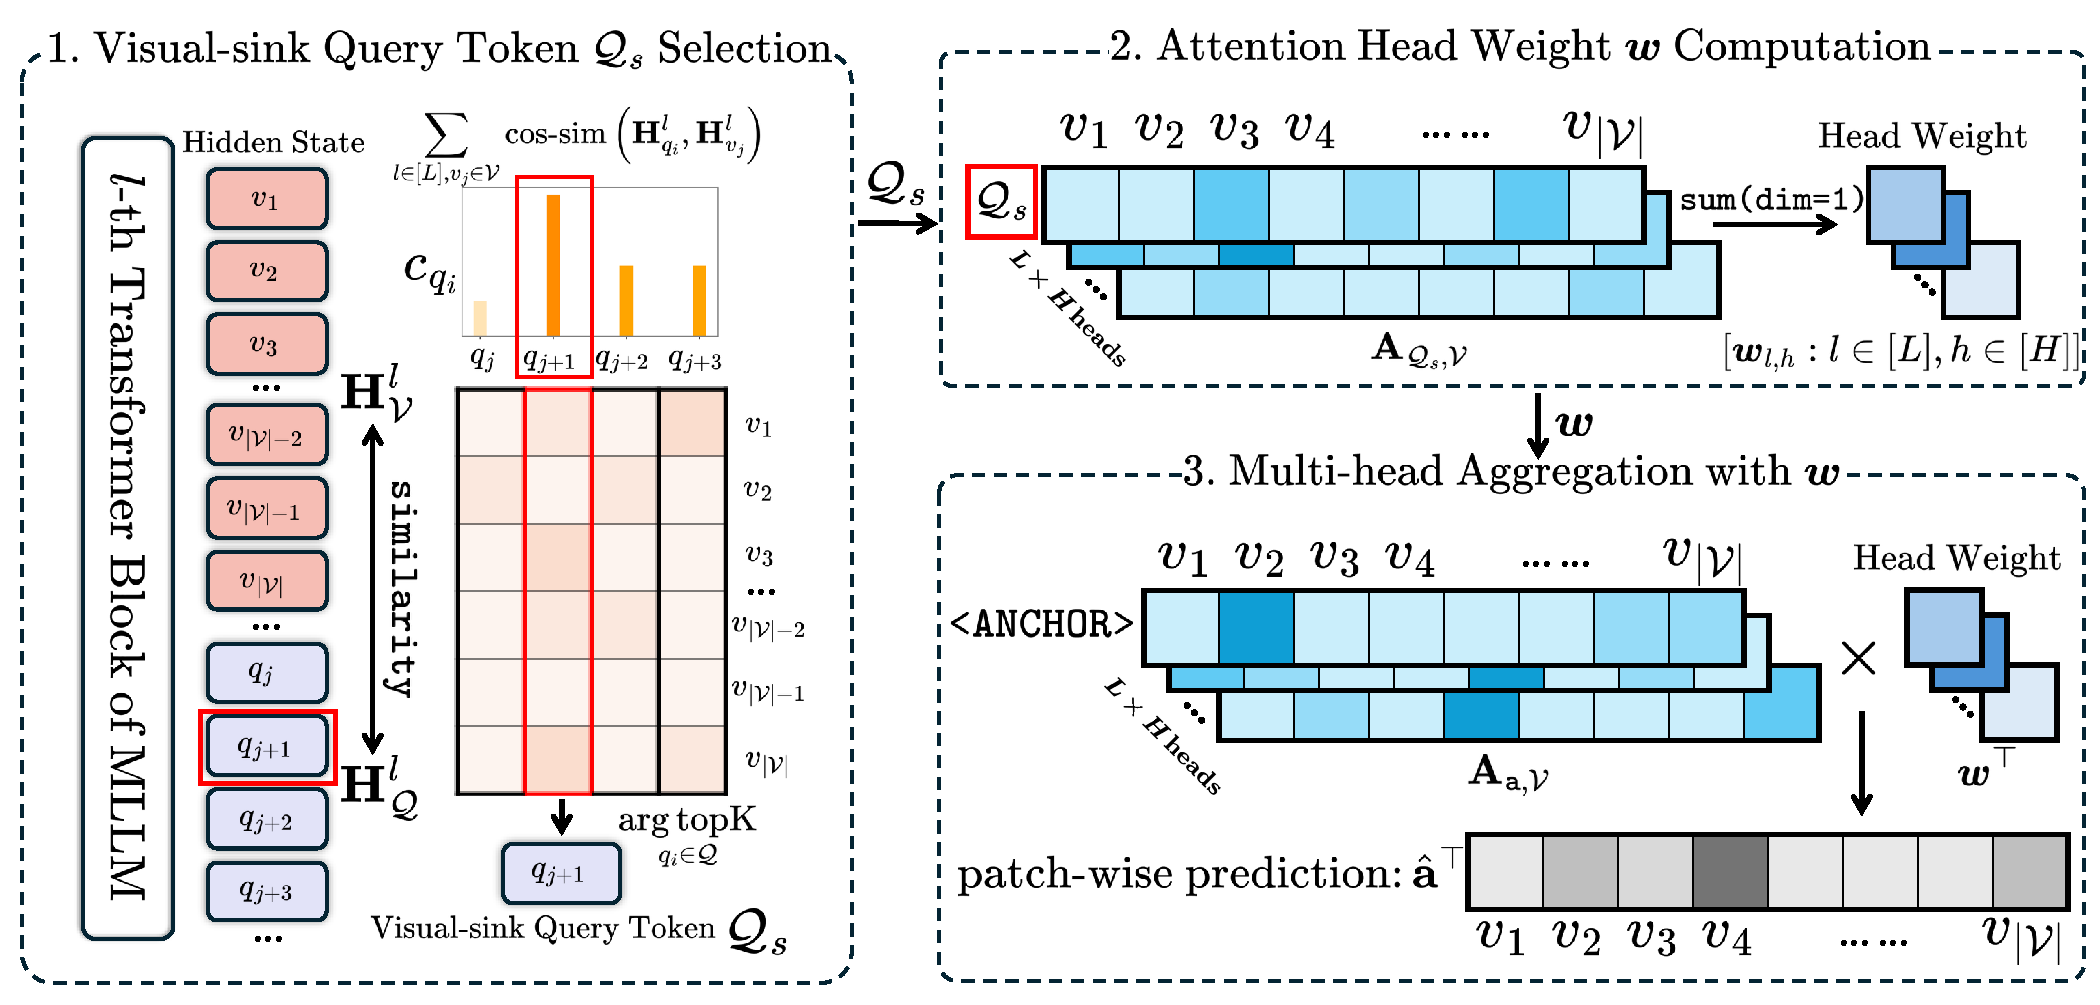
\includegraphics[width=0.95\linewidth]{fig/main_fig.pdf}
    % \vspace{-1em}
    \caption{Pipeline of \method{} for patch-wise prediction from the $\texttt{<ANCHOR>}$ token with attention-head weighting: \textbf{(i)} \method{} first selects visual-sink query tokens $\mathcal{Q}_s$ (\cref{eq:find_sink}) via computing hidden state similarities between query tokens and visual patches (\cref{eq:similarity}); \textbf{(ii)} it computes weights $\boldsymbol{w}$ of each attention head (\cref{eq:unified_head_score}) based on selected $\mathcal{Q}_s$; \textbf{(iii)} \method{} aggregates the grounding vectors of $\texttt{<ANCHOR>}$ token across layers and heads (\cref{eq:aggre_final}).} 
    % \vspace{-1.5em}
    \label{fig:main_fig}
\end{figure}
\subsection{Attention Head Weighting using Visual-sink Query Tokens} \label{sec:head_agg}
In \cref{sec:pre}, we introduce a special $\texttt{<ANCHOR>}$ token to avoid token-wise aggregation over all query words. We now discuss how to determine the head weights $w_{l,h}$ for the multi-head aggregation in \cref{eq:aggre_final}. 
Previous works~\citep{li2023inference,clark2019does} have shown the functional diversity between attention heads across transformer blocks in LLMs. For GUI grounding, we aim to emphasize heads that capture strong query-visual interactions, while down-weighting heads that mainly serve other functions. This selective weighting allows attention supervision to focus on grounding-relevant heads and to minimally perturb neutral heads, helping preserve pretrained capabilities.

\paragraph{An Attention-based View of Head Weighting.}
We measure the grounding relevance of each attention head by the amount of query-to-visual attention mass it carries: heads with stronger query-visual interactions are more likely to encode grounding-relevant correspondences.
For a selected query-side subset $\mathcal{Q}' \subseteq \mathcal{Q}\cup\{\texttt{<ANCHOR>}\}$, we define the head score of attention head $(l,h)$ as the cumulative attention mass from $\mathcal{Q}'$ to all visual tokens, with further normalization:
\begin{equation}
w_{l,h}(\mathcal{Q}')=\sum_{q\in\mathcal{Q}'}\sum_{v_j\in\mathcal{V}} \mathbf{A}^{l,h}_{q,v_j}, \quad w_{l,h}=\frac{\exp \left(w_{l,h}\right)}{\sum_{l'=1}^{L}\sum_{h'=1}^{H}\exp\!\big(w_{l',h'}\big)}
\label{eq:unified_head_score}
\end{equation}

Under this view, different head-weighting strategies can be unified by varying only the query-side token subset used to compute the score. A straightforward choice is to use all query tokens, i.e., $\mathcal{Q}'=\mathcal{Q}$. However, this choice is imprecise, since query tokens contribute unevenly to grounding, and aggregating over all of them can introduce noisy attention mass unrelated to the actual target region. Another simple choice is to use only the anchor token, i.e., $\mathcal{Q}'=\{\texttt{<ANCHOR>}\}$, since $\texttt{<ANCHOR>}$ serves as the representative token for grounding in \cref{eq:aggre_final}. Although simpler, this strategy can be unreliable early in training, because $\texttt{<ANCHOR>}$ is randomly initialized and may not yet serve as a stable context summarizer.

\paragraph{Visual-sink Query Token Selection.}
To estimate grounding-relevant head weights via  \cref{eq:unified_head_score}, we first identify a query-side token subset that captures query-visual interaction in a head-agnostic manner:
for a user query $\mathcal{Q}$, we estimate the visual affinity of each token $q_i$ at layer $l$, denoted as $c_{q_i}^l$, using cosine similarity between its hidden state and all visual patch states (Step~1 in \cref{fig:main_fig}). And We denote the selected top-K tokens via $c_{q_i}^l$ by $\mathcal{Q}_s$:
\begin{equation}
c_{q_i}^l=\sum_{v_j \in \mathcal{V}} \texttt{Sim}(\mathbf{H}^l_{q_i},\mathbf{H}^l_{v_j}).
\label{eq:similarity}
\end{equation}
A larger $c_{q_i}^l$ indicates that the representation of $q_i$ is more strongly aligned with the global visual context at layer $l$.

We use hidden-state similarity instead of directly relying on attention values because grounding-relevant query-visual interactions are often concentrated in only a subset of attention heads, and may therefore not be uniformly observable from raw attention patterns alone~\citep{elhelo2024inferring,olsson2022context,voita2019analyzing}. In contrast, the similarity score computed in \cref{eq:similarity} provides a head-agnostic and more global representation-space signal, making it more stable for identifying tokens that consistently correlate with cross-modal interaction, as shown in \cref{app:qs_analysis}.

\begin{wrapfigure}[14]{r}{0.6\textwidth}
  \vspace{-1.2\baselineskip} % 关键：把wrapfigure顶端抬到当前行
  \centering
  \setlength{\intextsep}{0pt}   
  \setlength{\columnsep}{0pt}   
  \setlength{\abovecaptionskip}{2pt}
  \setlength{\belowcaptionskip}{0pt}
  % \caption{Distribution of top-1 selected visual-sink query tokens under $c_{q_i}$.}
  % \vspace{-0.4em}
  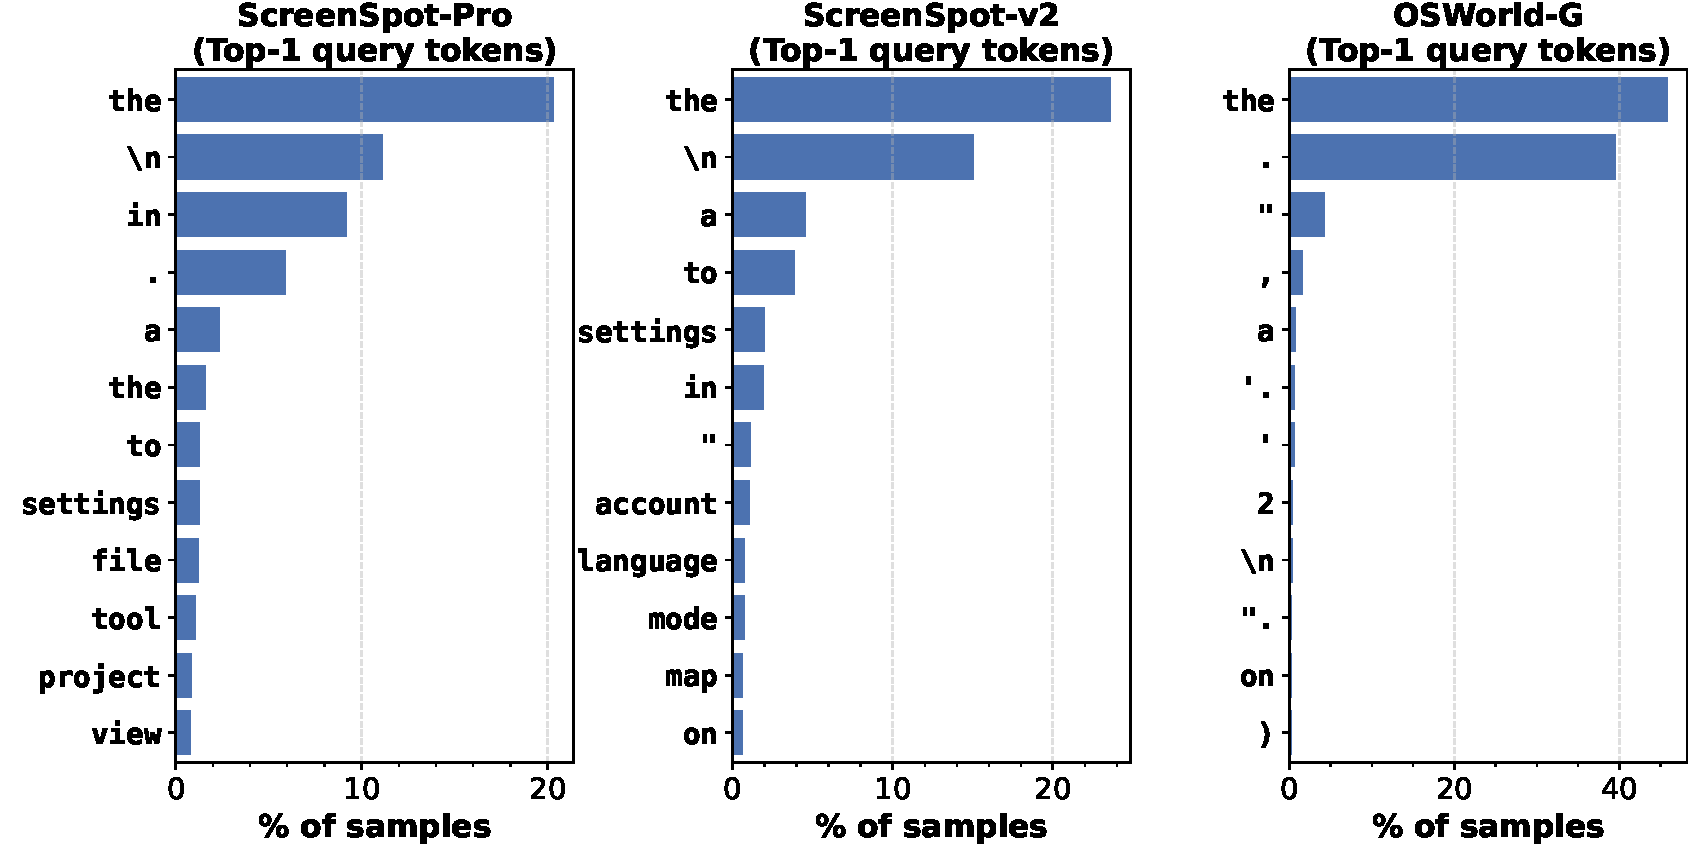
\includegraphics[width=\linewidth]{fig/query_top_tokens.pdf}
  \caption{Distribution of top-1 selected visual-sink query tokens under $c_{q_i}$.}
  % \vspace{-0.8em}
  \label{fig:top_tokens}
\end{wrapfigure}
As shown in \cref{fig:top_tokens}, the top-ranked token often shows a sink-like behavior: it repeatedly concentrates interaction with the visual context without necessarily being the most semantically informative word. We therefore refer to these tokens as \textbf{visual-sink query tokens}, emphasizing their role as \emph{functional proxies} for cross-modal interaction. In practice, we find that using a shared token set across all layers provides better stability and performance, instead of layer-wise $\mathcal{Q}_s^l$ for each layer as $\mathcal{Q}_s^l\coloneqq \operatorname*{arg\,topK}_{q_i\in\mathcal{Q}}(c_{q_i}^{\,l})$. Specifically, we adopt a \textbf{global uniform} selection that first aggregates $c_{q_i}^l$ across layers and then selects a shared visual-sink query token set $\mathcal{Q}_s$:
\begin{equation}
\mathcal{Q}_s
\coloneqq \operatorname*{arg\,topK}_{q_i\in\mathcal{Q}}(c_{q_i}),
\quad
c_{q_i}=\sum_{l=1}^{L} c_{q_i}^{\,l}.
\label{eq:find_sink}
\end{equation}

With $\mathcal{Q}_s$, we compute the normalized head weights $w_{l,h}$ using \cref{eq:unified_head_score}. Intuitively, if a head assigns substantial query-to-visual attention mass through these selected tokens, its attention pattern is more consistent with the cross-modal alignment pattern found in representation space. We therefore assign such heads larger weights in \cref{eq:aggre_final} to produce the final patch-level prediction $\hat{\mathbf{a}}$.

\subsection{Training and Inference Design}
\paragraph{Coordinate-free Supervision with Patch-wise Labels.} \label{sec:label}
Since our attention grounding is defined over visual patches rather than pixel coordinates, we convert each ground-truth bounding box $gt^{\mathrm{bbox}}=[x_1,y_1,x_2,y_2]$ into a patch-level label vector $\bm{p}\in\mathbb{R}^{|\mathcal{V}|}$, where $|\mathcal{V}|$ is the number of visual patches. A patch $v_i$ is assigned a positive label only if it overlaps with $gt^{\mathrm{bbox}}$.

To emphasize central patches while softly down-weighting partially overlapped boundary patches, we assign each positive patch a weight based on both its overlap with the ground-truth box and its distance to the box center, following GUI-$\text{G}^2$~\citep{tang2025gui}:
\begin{equation}
    p_{v_i}
    =\textbf{IoU}(v_i,gt^{\mathrm{bbox}})\cdot
    \mathcal{N}\!\left(\boldsymbol{\mu}_{v_i};\boldsymbol{\mu}_{gt},\boldsymbol{\Sigma}_{gt}\right),
    \label{eq:labeling}
\end{equation}
where $\boldsymbol{\mu}_{v_i}$ and $\boldsymbol{\mu}_{gt}$ denote the centers of patch $v_i$ and $gt^{\mathrm{bbox}}$, respectively, and
$\boldsymbol{\Sigma}_{gt}=\mathrm{diag}\!\left((\sigma_x^{gt})^2,(\sigma_y^{gt})^2\right)$ with
$\sigma_x^{gt}=\alpha(x_2-x_1)$ and $\sigma_y^{gt}=\alpha(y_2-y_1)$. 
% We set $\alpha=0.8$ empirically.

The final label vector is normalized as
$\bm{p}=\mathrm{normalize}(\{p_{v_i}\}_{i=1}^{|\mathcal{V}|})$,
which is both overlap-aware and center-biased. We then supervise the predicted patch distribution $\hat{\mathbf{a}}$ from \cref{eq:aggre_final} using the KL divergence:
\[
    \mathcal{L}_{\text{Attn}}=\mathbb{D}_{\mathrm{KL}}(\bm{p}\,\|\,\operatorname{normalize}(\hat{\mathbf{a}})).
\]

\paragraph{Two-step Inference with Zoom-in \faSearchPlus.} \label{sec:zoom}
Under GPU memory constraints, high-resolution GUI screenshots are usually down-sampled, yielding fewer visual patch tokens for the MLLM. The resulting information loss and reduced fine-grained spatial granularity inevitably harm grounding accuracy. 
\method{} provides flexible spatial granularity since its patch-wise grounding. We can easily perform a two-step inference by adding zoom-in \textbf{without extra training}: (1) feed the compressed high-resolution screenshot to predict the approximate location. We use the center of this predicted location to determine a specific area to focus on. (2) we re-run the inference on the newly cropped region, providing a much more accurate result. 
This two-step inference targets to mitigate failure cases on high-resolution screens where the model identifies the right region, but the center prediction is slightly offset from the ground-truth box. Detailed observations and analysis of the zoom-in strategy are provided in \cref{sec:zoomin_analysis}.

\paragraph{Efficient Attention Map Extraction.}
FlashAttention~\citep{dao2022flashattention} avoids materializing full attention maps, while standard eager attention~\citep{vaswani2017attention} can return them but is slower and more memory-intensive. In \method{}, we use FlashAttention for the regular forward pass and eager attention only for the grounding-relevant rows, i.e., the query tokens and $\texttt{<ANCHOR>}$ over visual tokens. This reduces the extraction cost roughly from $O((|\mathcal{V}|+|\mathcal{Q}|+1)^2)$ to $O((|\mathcal{Q}|+1)\cdot|\mathcal{V}|)$. Since $|\mathcal{Q}|\ll |\mathcal{V}|$ in typical GUI inputs, the additional overhead is negligible ($\sim$ 4.2\%). We provide analyses of inference efficiency in \cref{app:extra_res}.